% ============================================================
%  Chapter fragment -- included by main.tex
%  (not a standalone document; compile main.tex to build the PDF)
% ============================================================
\begin{multicols*}{3}
\raggedcolumns

\sheettitle{07 -- Exploitation \& ROP}{SWS2 -- ZHAW / Tellenbach}

\begin{defbox}
\hl{(!!) EXAM:} there will be \hl{at least one ROP question}: given a C program + a list of addresses (gadgets, .bss, strings, functions -- \kw{some irrelevant}) + junk buffers, \kw{put them in the right order} to achieve a stated goal. The recipe + worked example below are the heart of this chapter.
\end{defbox}

% ==================== DEFINITION / CLASSIFICATION ====================
\section{Exploits -- Definition \& Classification}
\kw{Exploit} = a \kw{piece of software}, \kw{chunk of data}, or \kw{sequence of commands} that takes advantage of a vulnerability $\to$ \kw{unintended/unanticipated behaviour}.
\begin{itemize}
\item \kw{Chunk of data}: \term{Ping of Death} (oversized IP packet crashes host). \kw{Software}: malicious JS in browser. \kw{Commands}: CVE-2017-5521 Netgear admin-pw recovery.
\item \kw{Human "hardware"} exploits = \kw{social engineering} (cognitive biases) $\to$ (spear) phishing, tailgating.
\end{itemize}
\subsection{Classification}
By \kw{action}: unauth data access, \kw{arbitrary code execution}, DoS, privilege escalation. 
Plus:

{\footnotesize
\setlength{\tabcolsep}{3pt}
\renewcommand{\arraystretch}{1.05}
\arrayrulecolor{zhawblue}
\noindent\begin{tabular}{@{}>{\raggedright\arraybackslash}p{0.27\linewidth}>{\raggedright\arraybackslash}p{0.65\linewidth}@{}}
\rowcolor{zhawblue}
{\color{white}\bfseries Term} & {\color{white}\bfseries Meaning}\\
\rowcolor{tableblue}
\kw{Local} & targets system it runs on (e.g. get admin).\\
\rowcolor{white}
\kw{Remote} & targets a \kw{remote} system.\\
\rowcolor{tableblue}
\kw{Client-side} & targets client SW, usually needs \kw{user help} (open file/site). \term{Drive-by} = no help (malicious ad).\\
\rowcolor{white}
\kw{Server-side} & targets a server, \kw{no user help} needed.\\
\rowcolor{tableblue}
\kw{0-day} & vuln \kw{not publicly known/patched} when exploited. \term{Day Zero} = day vendor/public learns of it.\\
\end{tabular}}
\textit{Our focus: \kw{memory-corruption} vulns to \kw{hijack control flow}.}

% ==================== MEMORY CORRUPTION ====================
\section{Memory Corruption Vulns \hl{(!)}}
\begin{itemize}
\item \kw{Buffer overflow}: no/wrong bounds-check, e.g. \term{char target[128]; strcpy(target, source)}.
\item \kw{Indexing errors}: can "jump over" areas (e.g. a \kw{stack canary}), no arbitrary control.
\item \kw{Arbitrary writes}: \term{array[user\_idx]=user\_data} with bad bounds.
\item \kw{Use-after-free}: use memory after \term{free()} (may be reused). \kw{Type confusion}.
\end{itemize}

% ==================== MEMORY ORGANISATION ====================
\section{Process Memory Layout \hl{(!)}}
Each process = own \kw{virtual address space}, split in \kw{segments}:
{\footnotesize
\setlength{\tabcolsep}{3pt}
\renewcommand{\arraystretch}{1.05}
\arrayrulecolor{zhawblue}
\noindent\begin{tabular}{@{}>{\raggedright\arraybackslash}p{0.27\linewidth}>{\raggedright\arraybackslash}p{0.65\linewidth}@{}}
\rowcolor{zhawblue}
{\color{white}\bfseries Segment} & {\color{white}\bfseries Holds}\\
\rowcolor{tableblue}
\kw{Stack} (high) & local vars, function params. \kw{Grows down}.\\
\rowcolor{white}
\kw{Heap} & dynamically allocated (\term{malloc}). Grows up.\\
\rowcolor{tableblue}
\kw{Data} & globals/statics (\kw{.bss} / .data).\\
\rowcolor{white}
\kw{Code} (low) & binary program code (\kw{.text}).\\
\end{tabular}}
\textit{\kw{.bss} = writeable global area -- handy as a \kw{scratch buffer} in ROP. \kw{.text} = executable code where \kw{gadgets} live.}
% >>> FIGURE: "Typical Memory Organisation" (slide 9): vertical stack/heap/data/code box. Good first illustration.

\begin{center}
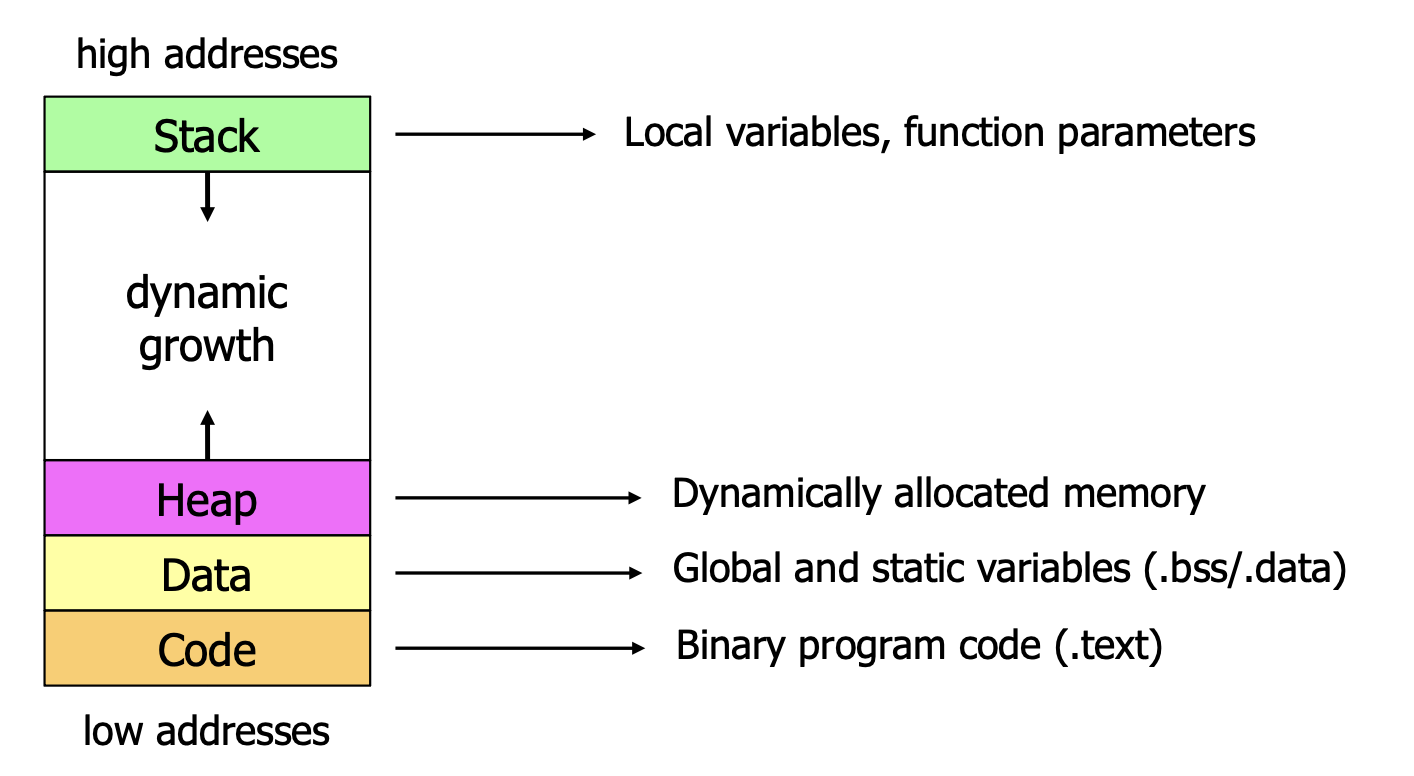
\includegraphics[width=0.9\linewidth]{Figures/memory_organisation.png}
\end{center}

% ==================== STACK & FUNCTION CALLS ====================
\section{Stack \& Function Calls (x86) \hl{(!)}}
% >>> FIGURE: "Stack Layout and Function Calls" (slide 10): parent/child frames with esp/ebp/ret addr -- very helpful here.
\subsection{The 3 key registers \hl{(!)}}
\begin{itemize}
\item \kw{ESP} (stack pointer) -- always points to the \kw{top of the stack} (most recently pushed item). Stack grows \kw{down} $\to$ ESP \kw{moves down on push, up on pop}. \textit{(= finger on the live edge of the plate stack.)}
\item \kw{EBP} (base / frame pointer) -- \kw{fixed reference} inside the current frame. ESP wanders as locals are pushed, but EBP \kw{stays put} $\to$ params/locals found at \kw{constant offsets} (\term{ebp+8}, \term{ebp-4}). \textit{(= bookmark stuck in the pile.)}
\item \kw{EIP} (instruction pointer) -- address of the \kw{next instruction} to execute. \hl{This is what the attacker wants to hijack} (overwrite ret addr $\to$ controls EIP).
\end{itemize}
\kw{32-bit cdecl}: args pushed on stack, \kw{caller cleans up}. A \kw{stack frame} (high$\to$low addr):
\begin{itemize}
\item \kw{...params} (param2 at \term{ebp+0Ch}, param1 at \term{ebp+8})
\item \kw{ret addr} (where to continue after the function) -- at \term{ebp+4}
\item \kw{saved ebp} (parent's ebp) $\leftarrow$ \term{ebp} points here
\item \kw{locals} (toward lower addr) $\leftarrow$ \term{esp} = top
\end{itemize}
\kw{At function entry}: \term{esp}$\to$ret addr, \term{esp+4}$\to$arg1, \term{esp+8}$\to$arg2 \dots \hl{(this is why ROP arg layout works)}.\\
\kw{Function epilogue}: \term{leave} (= \term{mov esp,ebp; pop ebp}) then \term{ret} (= \term{pop eip}, i.e. pop ret addr into EIP).

% ==================== BUFFER OVERFLOW ====================
\section{Stack Buffer Overflow -- Classic \hl{(!)}}
% >>> FIGURE: "Stack-Based Buffer Overflow" (slide 11): buffer before vs after code injection, red arrow ret addr -> buf. Great visual.

\begin{center}
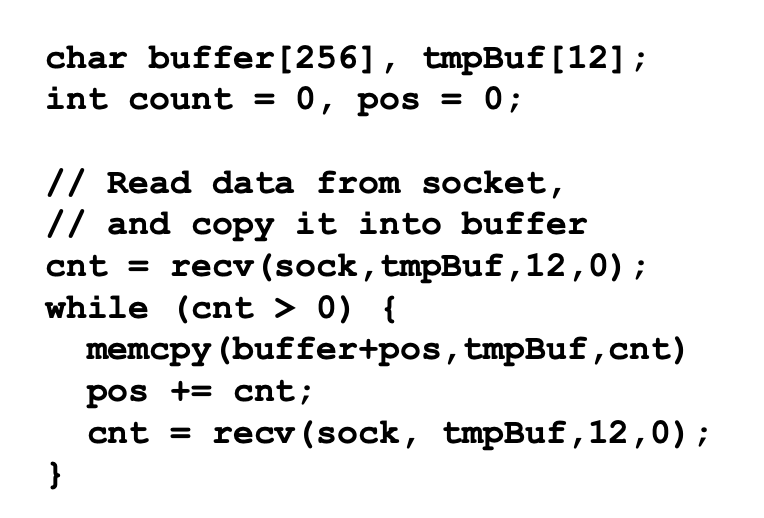
\includegraphics[width=0.5\linewidth]{Figures/buf_overflow_code.png}
\end{center}

\begin{center}
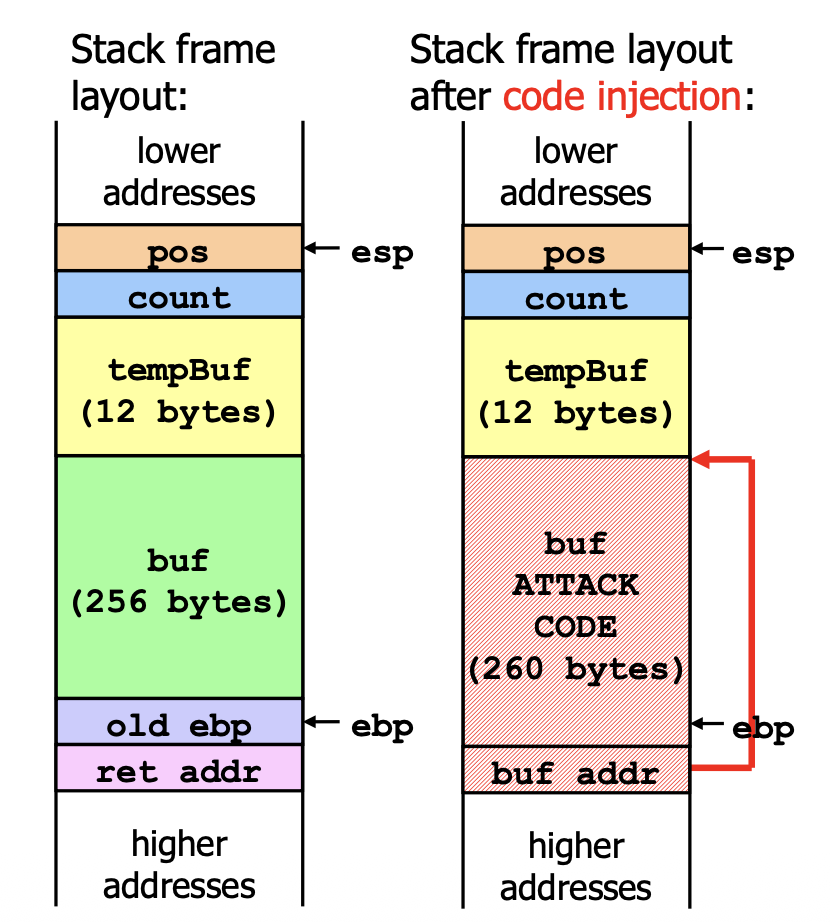
\includegraphics[width=0.5\linewidth]{Figures/buf_overflow_layout.png}
\end{center}

Write past a stack buffer $\to$ overwrite \kw{saved ebp} and \kw{ret addr}. \kw{Classic code injection}: fill buffer with \kw{shellcode}, overwrite ret addr with \kw{address of the buffer} $\Rightarrow$ on \term{ret}, EIP jumps into your shellcode on the stack.\\
\hl{This is exactly what NX/DEP kills} (stack not executable) $\Rightarrow$ need \kw{ROP}.

% ==================== PROTECTIONS ====================
\section{Protections (revisited) \hl{(!)}}
{\footnotesize
\setlength{\tabcolsep}{3pt}
\renewcommand{\arraystretch}{1.05}
\arrayrulecolor{zhawblue}
\noindent\begin{tabular}{@{}>{\raggedright\arraybackslash}p{0.24\linewidth}>{\raggedright\arraybackslash}p{0.68\linewidth}@{}}
\rowcolor{zhawblue}
{\color{white}\bfseries Protection} & {\color{white}\bfseries Idea / ROP impact}\\
\rowcolor{tableblue}
\kw{NX/DEP/XN} & mark pages \kw{non-executable} (NX=Linux, DEP=Win, XN=ARM). Stops stack shellcode. \hl{ROP defeats it} (reuses existing .text code).\\
\rowcolor{white}
\kw{ASLR} & randomise segment positions. Entropy \kw{low on 32-bit}, high on 64-bit. \hl{ROP needs gadget addresses} $\to$ ASLR hurts ROP.\\
\rowcolor{tableblue}
\kw{Stack canary} & random value before ret addr; checked in epilogue; \kw{sequential overwrite} of ret addr corrupts it $\to$ \term{\_\_stack\_chk\_fail}.\\
\end{tabular}}

% ============================================================
%  ROP
% ============================================================
\section{ROP -- Concept \hl{(!)}}
\kw{Return-Oriented Programming} (Krahmer 2005): \kw{execute arbitrary code WITHOUT injecting any code} -- reuse the \kw{application's own code}.
\begin{itemize}
\item \kw{Gadget} = a short existing instruction sequence \kw{ending in \term{ret}}. The \term{ret} passes control to the \kw{next} gadget/address on the stack (attacker-chosen).
\item \kw{Control-flow hijacking}: by laying out a \kw{sequence of addresses} on the stack, you \kw{chain gadgets/functions} like dominoes $\to$ build a new "program" out of existing pieces. Enough code exists in most binaries for any functionality.
\item \hl{NX/DEP is useless against ROP} (no new code runs). ROP does \kw{NOT} by itself beat \kw{ASLR} or \kw{canaries}.
\end{itemize}

\subsection{The vulnerable program}
\term{void target()\{printf("target");\}} = what we want to run. \term{void process\_arg(char* a)\{char buf[1024]; strcpy(buf,a);\}} $\leftarrow$ \kw{bug}: \term{strcpy} copies until a null byte, ignoring \term{buf}'s size. \term{main} calls \term{process\_arg(argv[1])}. A long \term{argv[1]} overflows \term{buf} up toward \kw{old ebp} \& \kw{ret addr}.\\
\hl{Why ROP not shellcode:} NX/DEP marks the stack non-executable $\Rightarrow$ shellcode in \term{buf} \kw{won't run}. ROP injects \kw{no code} -- only reuses existing (executable) code.

\subsection{Step 1 -- find the offset \hl{(!)}}
Need bytes from \term{buf} start to the ret-addr slot. Fill with 1024 A's, break after \term{strcpy}, read addresses with gdb \term{info frame}: \term{buf}=\term{0xffffcd00}, saved-eip slot=\term{0xffffd10c} $\Rightarrow$ \hl{0xffffd10c - 0xffffcd00 = 1036}. (1036, not 1024: \kw{old ebp} + alignment/saved regs sit between.)
\begin{center}
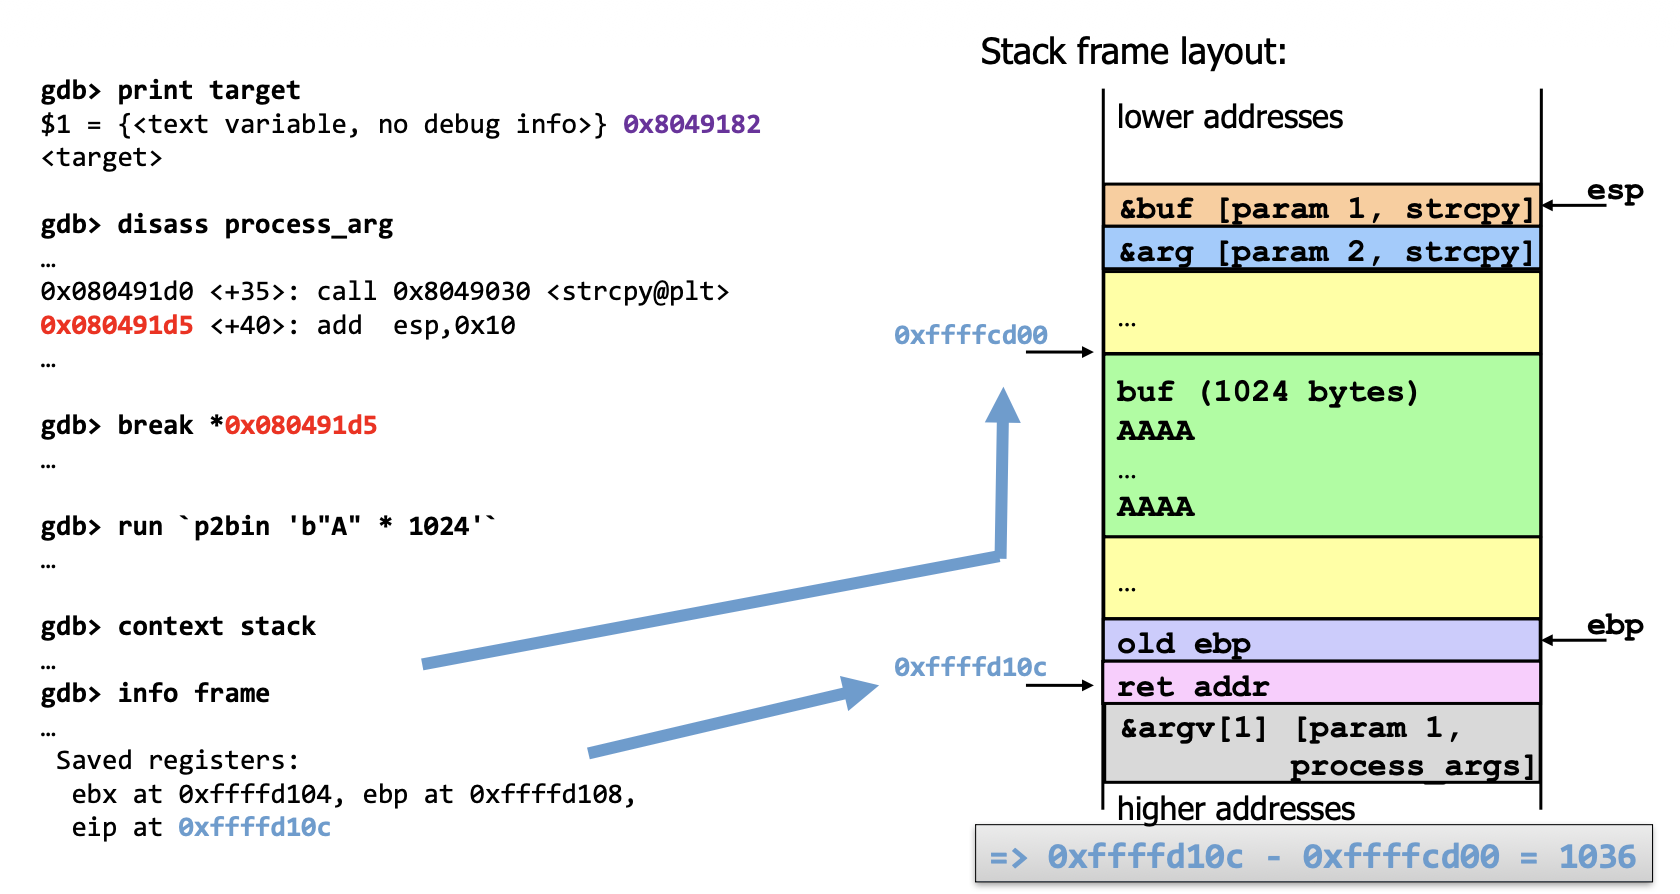
\includegraphics[width=0.95\linewidth]{Figures/stack_frame_1.png}
\end{center}

\subsection{Attempt 1 -- call target once}
Input: \term{b"A"*1036 + pack("<L", 0x08049182)} (1036 filler + 4-byte LE addr of \term{target} into ret slot). Trace \term{process\_arg} epilogue:
\begin{itemize}
\item \term{leave}: \term{esp=ebp}, then \term{pop ebp} reads the old-ebp slot = \term{0x41414141} (AAAA) $\to$ EBP = garbage (\kw{no crash yet}, nobody uses EBP).
\item \term{ret}: pops next slot = \term{0x08049182} into EIP $\to$ jumps to \term{target} $\Rightarrow$ \kw{prints "target"}. \kw{It works!}
\end{itemize}
\hl{But then:} \term{target} runs its own \term{leave;ret}; the slot now on top is \term{\&argv[1]} (leftover from \term{main}), \kw{not a code address} $\to$ EIP jumps into data $\to$ \kw{segfault}. \textit{Key insight: one call works, but you can't cleanly regain control afterward.}

\subsection{Attempt 2 -- chain target $\times$3}
\term{b"A"*1036 + \&target + \&target + \&target} $\Rightarrow$ "target target target", then segfault. \hl{Works only because \term{target} takes \kw{no args}}: each \term{ret} pops the next slot, which is conveniently the next \&target. \kw{0-arg functions chain trivially} (return slot = next function).

\subsection{The problem -- functions WITH params \hl{(!!)}}
% >>> FIGURE: "Calling Functions with Parameters" stack diagram (slide 26).
Goal: call \term{strcpy(dest,src)} (2 args) then \term{target}. In cdecl a function reads args \kw{just above its return addr}. So to call \term{strcpy} the stack needs: \kw{[\&strcpy][ret-addr-for-strcpy][arg1][arg2]}.\\
\hl{The conflict:} a single slot \kw{can't be both a return address AND an argument}. When \term{strcpy} does \term{ret}, it pops the slot right after its ret-addr slot = \kw{arg1} (\term{\&"\#args!"}) $\to$ EIP jumps into a \kw{data address} $\to$ \kw{segfault}. The args you placed sit exactly where the next return address must go.
\begin{center}
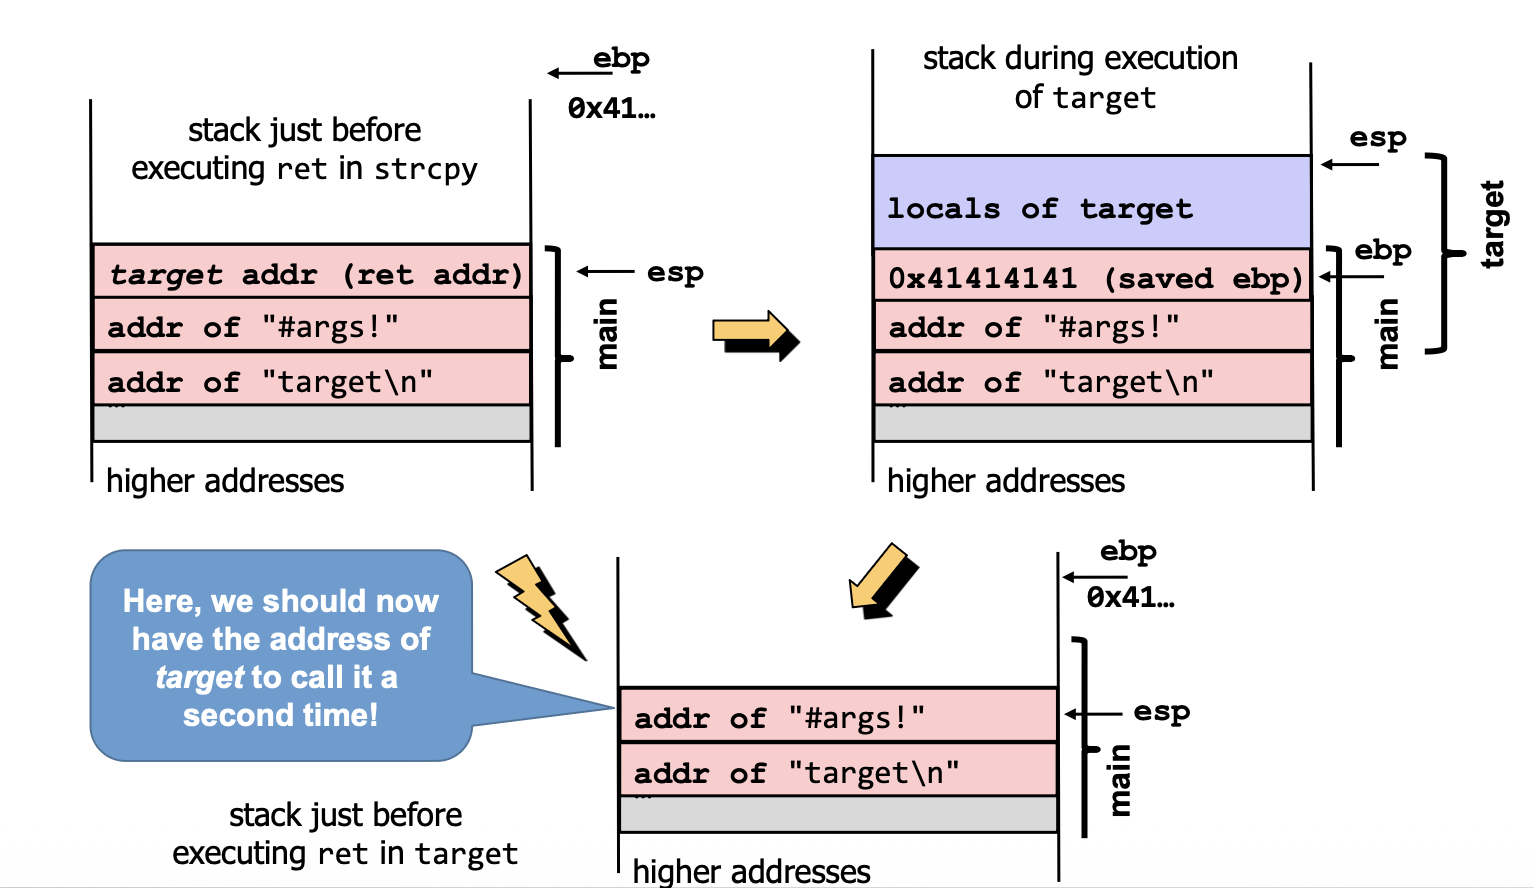
\includegraphics[width=0.95\linewidth]{Figures/stack_frame_params_func.png}
\end{center}

\subsection{Gadgets to the rescue $\to$ PPR \hl{(!!)}}
% >>> FIGURE: PPR gadget chaining (slide 30).
Between functions insert a \kw{gadget}: existing code that \kw{cleans args off the stack} then \term{ret}s. For a \kw{2-arg} function use \kw{pop;pop;ret} (\kw{PPR}): the 2 pops bump \term{esp} past arg1\&arg2 (into junk registers), then \term{ret} jumps to the next planted address. Trace:
\begin{itemize}
\item ret slot = \term{\&strcpy} $\to$ EIP enters \term{strcpy}; above it: \kw{PPR addr}, arg1, arg2.
\item \term{strcpy} returns $\to$ pops \kw{PPR addr} $\to$ enters gadget.
\item gadget \term{pop;pop} skips arg1\&arg2 $\to$ \term{ret} pops next = \term{\&target} $\to$ runs target.
\end{itemize}
\textit{PPR = the "glue" keeping the chain alive after a function eats its args.}
\begin{center}
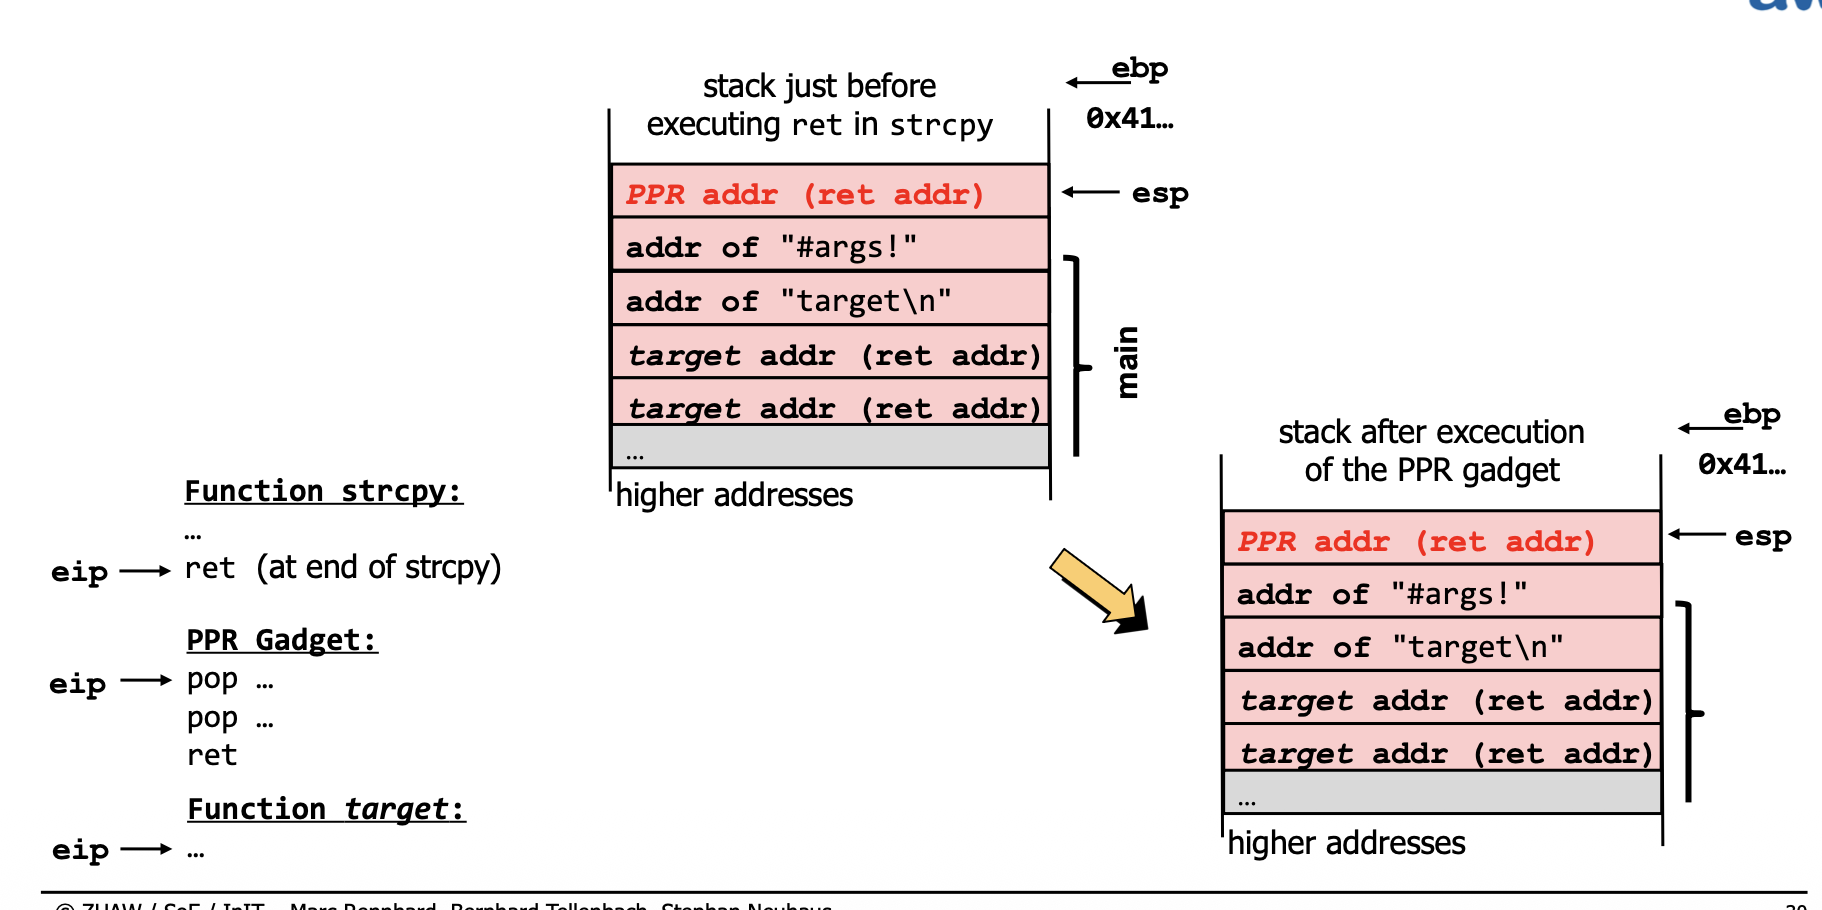
\includegraphics[width=0.95\linewidth]{Figures/stack_frame_gadgets.png}
\end{center}

\subsection{Final payload}
\term{b"A"*1036 + \&strcpy + \&PPR + \&"\#args!" + \&"target" + \&target + \&target}\\
Read top-to-bottom = "run \term{strcpy} with 2 args, clean up, run \term{target}, run \term{target}" -- a program written from \kw{borrowed pieces}. \hl{Rule:} func with \kw{N args} $\to$ insert \kw{N-pop + ret} gadget as its ret addr (\kw{PPR}=2 args, \kw{PR}=1, \kw{none}=0 args).

% ==================== GENERIC PATTERN ====================
\section{ROP -- Generic Recipe \hl{(!!)}}
\begin{defbox}
\kw{Stack layout (low$\to$high address = order bytes appear in payload):}\\
{\footnotesize
\setlength{\tabcolsep}{3pt}
\arrayrulecolor{zhawblue}
\noindent\begin{tabular}{@{}>{\raggedright\arraybackslash}p{0.34\linewidth}>{\raggedright\arraybackslash}p{0.58\linewidth}@{}}
\rowcolor{tableblue}
\kw{FILLER} & junk to reach \& overwrite \kw{EIP/ret addr}\\
\rowcolor{white}
\kw{FUNC\_1} & 1st function called (overwrites EIP)\\
\rowcolor{tableblue}
\kw{gadget (N\textsubscript{1} pops + ret)} & FUNC\_1's "ret addr"; \kw{N\textsubscript{1} = \#args of FUNC\_1}\\
\rowcolor{white}
\kw{ARG1\_F1, ARG2\_F1, \dots} & args for FUNC\_1\\
\rowcolor{tableblue}
\kw{FUNC\_2} & next function (gadget's ret lands here)\\
\rowcolor{white}
\kw{gadget (N\textsubscript{2} pops + ret)} & FUNC\_2's "ret addr"\\
\rowcolor{tableblue}
\kw{ARG1\_F2, \dots} & args for FUNC\_2\\
\rowcolor{white}
\kw{FUNC\_3 \dots} & \dots (or \term{exit()} for clean end)\\
\end{tabular}}
\end{defbox}
\hl{Key rule:} after every function with args, insert a \kw{pop$\times$(\#args) + ret} gadget as its return address. \kw{0-arg} functions need \kw{no} cleanup gadget (chain directly). \kw{Match \#pops to \#args.}

% ==================== WORKED EXAM EXAMPLE ====================
\section{Worked Exam-Style Example \hl{(!!)}}
\textit{Given addresses (note: in a real exam \kw{some are decoys}):}
{\footnotesize
\setlength{\tabcolsep}{3pt}
\arrayrulecolor{zhawblue}
\noindent\begin{tabular}{@{}>{\raggedright\arraybackslash}p{0.27\linewidth}>{\raggedright\arraybackslash}p{0.65\linewidth}@{}}
\rowcolor{zhawblue}
{\color{white}\bfseries Addr} & {\color{white}\bfseries Description}\\
\rowcolor{tableblue}
\term{0xaaaaaaaa} & \term{get\_data\_from\_ip(buf, maxlen, ip, port)} -- \kw{4 args}\\
\rowcolor{white}
\term{0xbbbbbbbb} & \term{save\_buffer(name, length, buf)} -- \kw{3 args}\\
\rowcolor{tableblue}
\term{0xcccccccc} & gadget \kw{PPPPR} (pop$\times$4; ret)\\
\rowcolor{white}
\term{0xdddddddd} & \kw{.bss} (writeable, $\ge$65536 bytes)\\
\rowcolor{tableblue}
\term{0xeeeeeeee} & gadget \kw{PPPR} (pop$\times$3; ret)\\
\rowcolor{white}
\term{0xffffffff} & string \term{"/tmp/abcdef"}\\
\end{tabular}}

\kw{Goal:} download \kw{8192 (0x2000)} bytes from IP \term{16.16.16.16 (0x10101010)} port \term{443 (0x1bb)}, then \kw{write to disk}. (This example: \kw{only the ROP chain}, no filler.)\\
\kw{Plan:} (1) \term{get\_data\_from\_ip}(.bss, 8192, ip, port) to fill .bss; (2) \term{save\_buffer}("/tmp/abcdef", 8192, .bss) to write it out.\\
\hl{Solution (payload top$\to$bottom):}


{\footnotesize
\setlength{\tabcolsep}{3pt}
\arrayrulecolor{zhawblue}
\noindent\begin{tabular}{@{}>{\raggedright\arraybackslash}p{0.30\linewidth}>{\raggedright\arraybackslash}p{0.62\linewidth}@{}}
\rowcolor{tableblue}
\term{0xaaaaaaaa} & FUNC\_1 = \term{get\_data\_from\_ip}\\
\rowcolor{white}
\term{0xcccccccc} & \kw{PPPPR} (cleans 4 args) = F1 ret addr\\
\rowcolor{tableblue}
\term{0xdddddddd} & arg1 buf = .bss\\
\rowcolor{white}
\term{0x00002000} & arg2 maxlen = 8192\\
\rowcolor{tableblue}
\term{0x10101010} & arg3 ip\\
\rowcolor{white}
\term{0x000001bb} & arg4 port\\
\rowcolor{tableblue}
\term{0xbbbbbbbb} & FUNC\_2 = \term{save\_buffer}\\
\rowcolor{white}
\term{0xeeeeeeee} & \kw{PPPR} (cleans 3 args) = F2 ret addr\\
\rowcolor{tableblue}
\term{0xffffffff} & arg1 name = \term{"/tmp/abcdef"}\\
\rowcolor{white}
\term{0x00002000} & arg2 length = 8192\\
\rowcolor{tableblue}
\term{0xdddddddd} & arg3 buf = .bss\\
\rowcolor{white}
\multicolumn{2}{@{}l}{\footnotesize\textit{-- optional clean-exit tail (only if asked) --}}\\
\rowcolor{tableblue}
\term{\&exit} & call \term{exit()} $\to$ process ends cleanly\\
\rowcolor{white}
\term{0x43434343} & exit's ret addr (\kw{junk}, exit never returns)\\
\rowcolor{tableblue}
\term{0x01010101} & arg = \kw{exit code} (\hl{no \term{0x00}} -- strcpy stops at null)\\
\end{tabular}}
\hl{Reasoning to remember:} \kw{4-arg} func $\to$ \kw{PPPPR}; \kw{3-arg} func $\to$ \kw{PPPR} (\#pops = \#args). \kw{Args} = read by the function (input); the \kw{gadget} then \kw{removes those same arg slots} (= the caller's missing \term{add esp}) so \term{ret} reaches the \kw{next} function. Reuse \kw{.bss} as the shared buffer (write then read). Pass \kw{values} for ints (ip/port/len), \kw{addresses} for pointers (buf, name string).\\
\hl{Clean exit:} \term{exit()} is a \kw{function you call} (\term{\&exit} + junk-ret + exit-code). It \kw{needs no cleanup gadget} (process ends $\to$ no next function). \term{0x01010101} is the \kw{exit code}, not the exit itself. \textit{(This example said "don't exit cleanly" $\to$ tail optional; the lab required it.)}

% ==================== LAB-STYLE FULL EXPLOIT ====================
\section{Full Exploit -- Lab (canary+DEP+ASLR) \hl{(!)}}
\textit{Vuln: struct \term{foo\_t} = \term{buf[128]} then func-ptr \term{cb}; \term{strcpy} into buf overflows into \term{cb}. \hl{Canary protects ret addr, NOT struct members} $\Rightarrow$ overwrite \term{cb} to bypass canary.} Goal: call \term{unused()} twice then \term{exit()} cleanly.
\begin{itemize}
\item \kw{Stack pivot}: overwrite \term{cb} with a \kw{leave;ret} gadget. \term{leave}=\term{mov esp,ebp; pop ebp} \kw{teleports ESP} to the (overwritten) saved-EBP area = our controlled data $\to$ chain runs; \hl{vuln's epilogue (canary check) is never reached}.
\item \kw{pop ebx;ret} gadget = the \kw{argument-skipper} (PR): after \term{unused()} returns, it discards the just-used arg then \term{ret}s to the next call.
\item \kw{Avoid null bytes}: \term{strcpy} stops at \term{0x00}, so use e.g. exit code \term{0x01010101} not \term{0x00000001}.
\end{itemize}
\kw{How 3 protections fell:} \kw{canary} -- pivot skips the epilogue check; \kw{DEP} -- no stack code, only existing .text; \kw{ASLR} -- binary built \term{-no-pie} (fixed addresses).

% ==================== DEFEATING CANARIES ====================
\section{Defeating Stack Canaries \hl{(!)}}
Canary blocks using the \kw{ret addr} for hijack. Alternative entry points:
\begin{itemize}
\item Overwrite a \kw{function pointer} (on stack or in a struct) $\to$ point to a gadget that \kw{adjusts ESP} to the top of your buffer; its \term{ret} starts the chain. \textit{(= the lab's leave;ret pivot.)}
\item \kw{Jump over} the canary (indexing bug). \kw{Leak} the canary (info-leak vuln). Overwrite \kw{SEH} (Windows).
\item \hl{Canary's LSB is \term{0x00}} (string terminator) -- known, but \term{strcpy} can't write a mid-payload \term{0x00} to restore it. \term{memcpy}/\term{memset} \kw{don't stop at null} $\to$ canary's null gives no protection there.
\end{itemize}

% ==================== DEFEATING ASLR ====================
\section{ROP vs ASLR -- "Is ROP dying?" \hl{(!)}}
ROP needs \kw{gadget addresses}. If \kw{all} code is ASLR'd, get \kw{at least ONE} address via \kw{info leak} or \kw{brute force} (\hl{32-bit entropy often low enough to brute-force} -- see lab).
\begin{itemize}
\item \hl{Why only one?} The code \kw{segment moves as a block} but its \kw{internal layout is fixed} $\to$ with a binary copy you \kw{compute all other gadgets} from one known address (relative offsets).
\item \kw{PIE/PIC}: modern OS compile critical binaries \kw{position-independent} (often default) so ASLR also randomises the main binary. (\kw{ASLR != ASLR}: "compiler default YES" $\ne$ "all programs use it"; embedded/IoT often lack DEP/ASLR.)
\item \kw{ROP fading?} To beat full ASLR you must \kw{read/leak memory} anyway -- and if you can read, you can often \kw{write} $\to$ "\term{Write Once, Pwn Anywhere}", \kw{no ROP needed}. Modern exploits often skip ROP (JIT-spray, corrupt a \term{safemode} flag, etc.). \kw{Importance decreasing} on general-purpose OS -- but \kw{IoT}?
\end{itemize}

% ==================== CFI / CFG ====================
\section{Control-Flow Integrity / Guard \hl{(!)}}
\kw{CFI / Control Flow Guard (CFG)} (Clang; Win 8.1/10, \term{/guard:cf}): app compiled with instrumentation that \kw{validates indirect calls} against a set of \kw{legal targets} $\to$ \kw{detects function-pointer overwrites} (call to \term{0x41414141} $\to$ terminate). \hl{Limit:} doesn't stop a vuln that drives a \kw{valid} code path with attacker data (e.g. forcing the "admin" path as a normal user).

% ==================== SUMMARY ====================
\section{Summary \hl{(!)}}
\begin{defbox}
\kw{ROP} = chain \kw{gadgets} (existing code ending in \term{ret}) by laying \kw{addresses on the stack} $\Rightarrow$ \kw{bypasses NX/DEP} without injecting code. \hl{Recipe:} FILLER $\to$ FUNC\_1 $\to$ \kw{pop$\times$(\#args)+ret} cleanup $\to$ args $\to$ FUNC\_2 $\to$ \dots ; \kw{\#pops = \#args}; \term{exit()} for clean end. ROP does \kw{not} solve \kw{ASLR}/\kw{canaries} (defeat those via \kw{info-leak / brute force / fn-ptr pivot}). \kw{CFI} \& ASLR raise the bar; ROP's importance is \kw{declining} on PCs (but not IoT).
\end{defbox}

\end{multicols*}
